\chapter{Introduzione}
Nel corso di questa trattazione andremo ad affrontare i temi fondamentali nello
studio delle reti di calcolatori.

\section{Struttura di internet}
Parlando di reti, la prima cosa che viene in mente è certamente internet, la rete
per antonomasia. La rete internet, in realtà, non è una singola rete, ma è
definita come la \emph{rete di tutte le reti}.

Questo può far venire il sospetto che le reti di calcolatori siano strutture in
qualche modo. Infatti è così! Internet è organizzato in una struttura
gerarchica, al cui vertice, o nucleo, troviamo gli \emph{\gls{glos:ISP} di
livello 1}, al livello inferiore gli \emph{ISP di livello 2}, poi gli \emph{ISP
di livello 3} e per finire, al livello più basso, si collocano gli
\emph{\gls{glos:host}}, ovvero i \emph{dispositivi terminali} degli utenti.

Ma cosa sono gli \emph{ISP}? Un \emph{ISP} è un \emph{Internet Service Provider},
cioè una società o un ente che mette a disposizione l'infrastruttura necessaria
a comunicare con altri utenti della rete. Ma vediamone meglio le differenze:
\begin{enumerate}
    \item \emph{ISP di livello 1}: (Telecom, AT\&T, \dots) sono pochi enti
    distribuiti nel mondo, ma che hanno una copertura nazionale/internazionale.
    Sono fittamente interconnessi e comunicano come pari;
    \item \emph{ISP di livello 2}: (Vodafone, Tim, \dots) sono enti che si
    appoggiano all'infrastruttura di uno o più \emph{ISP di livello 1} e hanno
    una copertura distrettuale/nazionale. Possono comunicare soltanto con gli
    \emph{ISP} dei quali sfruttano l'infrastruttura;
    \item \emph{ISP di livello 3}: sono le cosiddette \emph{reti di ultimo
    salto} o \emph{reti di accesso} e permettono agli utenti finali di accedere
    alla rete e quindi hanno una copertura locale;
\end{enumerate}

\paragraph{Internet Exchange Point}
Gli \emph{ISP di livello 2} possono comunicare direttamente tra loro, senza scalare
la gerarchia, attraverso punti particolari della rete detti \emph{\gls{glos:IXP}},
\emph{Internet Exchange Point}. Questi sono luoghi in cui le infrastrutture di
due o più \emph{ISP di livello 2} sono messe in comunicazione, permettendo così
al traffico dati di passare da un'infrastruttura all'altra. Questo tipo di
interscambi consentono, come vedremo, di ridurre il tempo necessario per il
trasferimento dei dati.

\paragraph{Reti single-homed e multi-homed}
Gli \emph{ISP di livello 3} possono appoggiarsi a uno o più \emph{ISP di livello
di 2}. Nel primo caso configurano una \emph{single-homed network}, mentre nel
secondo una \emph{multi-homed network}.

\subsection{Nucleo della rete}
La struttura gerarchica appena descritta permette di distinguere due livelli
della rete: un \emph{nucleo} e una \emph{periferia}.

Il \emph{nucleo} corrisponde alla parte di rete gestita dagli \emph{ISP di livello
1 e 2}, cioè la parte di infrastruttura non direttamente accessibile dagli utenti.
È evidente che questa parte della rete è quella in cui circola la maggior parte
del traffico, per cui rallentamenti, congestioni e guasti hanno conseguenze più
gravi. Per questo motivo, i dispositivi fisici che compongono
l'infrastruttura, oltre che essere più performanti delle loro controparti di
\emph{periferia}, sono collegati tramite strutture magliate. Ciò significa che
tra due dispositivi esistono una pluralità di collegamenti e percorsi possibili.
Questa ridondanza permette di ridurre il rischio di interruzioni del servizio, ma
anche di distribuire il traffico in maniera più efficiente, evitando che si
concentri su un unico punto.

\subsection{Periferia della rete}
La parte \emph{periferica} di internet corrisponde alla somma delle
\emph{reti di accesso}, cioè alla parte di competenza degli \emph{ISP di livello
3}. Questa parte della rete funge da interfaccia di collegamento per gli utenti
e i dispositivi terminali, cioè inoltra verso il \emph{nucleo} i dati da
trasmettere e riceve i dati in arrivo per poi occuparsi di farli arrivare
all'\emph{host} o al gruppo di \emph{host} destinatari.

Esistono diversi tipi di \emph{reti d'accesso} che si distinguono per la
dimensione e le tecnologie utilizzate.
Dividendole per dimensione si hanno:
\begin{itemize}
    \item \emph{Reti d'accesso residenziali}: coprono l'area di un'abitazione;
    \item \emph{Reti d'accesso aziendali}: coprono l'area di più edifici, o di
    un campus;
\end{itemize}

\noindent
Suddividendole invece per tecnologia si hanno:
\begin{itemize}
    \item \emph{Reti d'accesso punto-punto}: i dispositivi sono connessi
    direttamente, o attraverso uno \emph{\gls{glos:switch}} al 
    \emph{\gls{glos:router}}. È possibile un'ulteriore suddivisione:
    \begin{itemize}
        \item \emph{Reti con modem dial-up}: è una tecnologia vecchia e lenta
        che sfrutta i collegamenti telefonici in maniera esclusiva, cioè non
        permette di telefonare e accedere alla rete in contemporanea;
        \item \emph{Reti \gls{glos:DSL}}: sfrutta anch'essa i collegamenti
        telefonici, ma non in modo esclusivo;
        \item \emph{Reti \gls{glos:FTTH}}: il \emph{router} locale è connesso
        all'\emph{ISP di livello 2} tramite collegamenti in \emph{fibra ottica}
        molto veloci;
    \end{itemize}
    \item \emph{Reti d'accesso wireless}: usano tecnologie wireless e tanti utenti
    si connettono allo stesso punto, detto \emph{base station} o \emph{access point},
    il quale è connesso a un \emph{router};
\end{itemize}

\section{Mezzi trasmissivi}
All'interno delle reti, le informazioni, codificate in bit, viaggiano su dei
\emph{mezzi trasmissivi}. Ne esistono di tipologie diverse:
\begin{itemize}
    \item \emph{Mezzi guidati}: i segnali si propagano su un mezzo \emph{fisico}
    \begin{itemize}
        \item \emph{Doppini intrecciati}: è un cavo costituito da due fili di rame
        intrecciati;
        \item \emph{Cavi coassiali}: è un cavo costituito da un'anima centrale di
        rame e una maglia costituita da cavi metallici intrecciati. L'anima e la
        maglia sono separati da uno strato isolante;
        \item \emph{Fibra ottica}: l'informazione viaggia sotto forma di impulsi
        luminosi e questa è la soluzione ottimale per le lunghe distanze;
    \end{itemize}
    \item \emph{Mezzi a onda libera}: i segnali si propagano attraverso l'atmosfera
    e lo spazio esterno sfruttando i campi elettromagnetici
    \begin{itemize}
        \item \emph{Reti a microonde terrestri};
        \item \emph{Reti Wi-Fi}: le più usate nelle \emph{reti locali};
        \item \emph{Reti cellulari}: le più usate per la mobilità;
        \item \emph{Reti satellitari}: sono ottimali per le lunghe distanze e per
        luoghi che non hanno accesso a \emph{reti cellulari};
    \end{itemize}
\end{itemize}
I \emph{mezzi a onda libera} esaltano la mobilità, in quanto non è richiesto un
collegamento fisico con il punto d'accesso alla rete, ma sono maggiormente soggetti
a problemi di interferenze e riflessioni dei segnali. Per i \emph{mezzi guidati}
vale il contrario.

\subsection{Doppini intrecciati}
Esaminiamo più a fondo i \emph{doppini intrecciati} che sono quelli tipicamente
usati nello standard \emph{Ethernet}. Un cavo di questo tipo è formato da 4
coppie di fili di rame intrecciati detti \emph{doppini}.

Per evitare problemi di interferenza tra i cavi o i singoli \emph{doppini} è
possibile usare delle schermature. Diverse configurazione delle schermature sono
codificate con un sistema di lettere:
\[X/YTP\]
dove $X$ indica il tipo di schermatura del cavo e $Y$ la schermatura dei singoli
doppini.
\newline Schermatura del cavo:
\begin{itemize}
    \item \emph{U}: unshilded;
    \item \emph{F}: foiled (rivestito con una lamina di alluminio);
    \item \emph{S}: rivestito con una maglia metallica (rame placcato in alluminio);
    \item \emph{SF}: entrambe;
\end{itemize}
Schermatura dei \emph{doppini};
\begin{itemize}
    \item \emph{U}: unshilded;
    \item \emph{F}: shielded;
\end{itemize}

\paragraph{Cavi patch VS cavi cross}
Nello standard \emph{Ethernet}, nelle prese \emph{RJ45}, i 4 \emph{doppini} sono
collegati ai pin della presa mettendoli in riga affiancati. Nei \emph{cavi patch}
l'ordine dei \emph{doppini} è uguale a entrambi i capi del cavo, mentre nei cavi
\emph{cross} i due \emph{doppini} esterni sono scambiati di posizione e allo
stesso modo sono scambiati anche i \emph{doppini} interni.

\section{Tecniche di commutazione}
Abbiamo detto come i bit di dati viaggino da un dispositivo a un altro, ma non
abbiamo ancora chiarito come siano organizzati questi trasferimenti. Ciò è definito
dalla \emph{tecnica di commutazione} utilizzata. Ne esistono due:
\begin{itemize}
    \item \emph{Commutazione di circuito}: prima del trasferimento viene stabilito
    a priori il percorso che il messaggio dovrà seguire;
    \item \emph{Commutazione a pacchetto}: il messaggio viene scomposto in pacchetti
    che attraversano la rete in modo indipendente gli uni dagli altri;
\end{itemize}

\subsection{Commutazione di circuito}
Come accennato, questa \emph{tecnica di commutazione} prevede che il messaggio
venga trasmesso in blocco e che le risorse necessarie a collegare mittente e
destinatario siano riservate per quella comunicazione.

Ad essere suddivisa in porzioni è l'\emph{ampiezza di banda} (il \emph{bandwidth})
secondo 3 parametri:
\begin{enumerate}
    \item \emph{Bit rate}: e.g. in una rete a $10\frac{Mb}{s}$ vengono creati due
    canali da $5\frac{Mb}{s}$ che vengono assegnati a due utenti senza un limite
    di tempo;
    \item \emph{Frequenza}: (\emph{\gls{glos:FDM}}) la frequenza
    viene suddivisa in più canali che vengono assegnati agli utenti senza un limite
    di tempo;
    \item \emph{Tempo}: (\emph{\gls{glos:TDM}}) ogni utente ha a
    disposizione per un tempo limitato tutta la frequenza del canale;
\end{enumerate}

\begin{figure}[h]
    \centering
    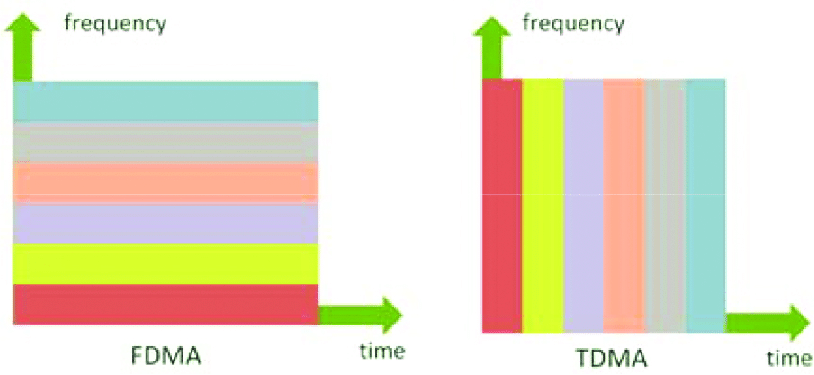
\includegraphics[width=\textwidth]{images/fdm-tdm.png}
    \caption{\emph{FDM} VS \emph{TDM}}
\end{figure}\noindent
Il vantaggio di questo tipo di \emph{commutazione} è che ogni utente al quale è
stato assegnato un canale (o slot) sa quali risorse avrà a disposizione. Tuttavia,
queste risorse devono essere negoziate prima della trasmissione e quindi è prevista
una fase di \emph{handshake} nella quale vengono prenotate e assegnate le risorse.
Inoltre, quando l'utente non le usa, quelle risorse sono sprecate.

\subsection{Commutazione a pacchetto}
Diversamente da prima, qui il messaggio viene suddiviso in pacchetti di uguale
dimensione (tipicamente 1.5MB) che vengono trasmessi singolarmente. Nel momento
della trasmissione, il pacchetto utilizza tutta la banda del canale che non viene
quindi ripartita tra gli utenti, ma condivisa. In questo modo, l'uso delle
risorse avviene a seconda delle necessità e, infatti, questa \emph{tecnica di
commutazione} è adatta per situazioni in cui un utente utilizza la rete soltanto
per pochi istanti.

Questa tecnica è soggetta a problemi di \emph{congestione} provocata dall'accodamento
dei pacchetti in attesa di essere trasmessi e ciò è anche diretta conseguenza
del comportamento dei commutatori. I commutatori infatti, prima di trasmettere un
pacchetto devono riceverlo per intero. Per questo motivo in ogni commutatore esiste
un buffer nel quale vengono memorizzati i pacchetti in attesa di essere
trasmessi e, quando questo è pieno, i nuovi pacchetti in arrivo vengono scartati.

Questo problema di perdita dei pacchetti viene risolto (se serve!) da determinati
protocolli che verranno trattati più avanti.

\paragraph{Ritardi nelle trasmissioni}
Nella comunicazione in rete, specie con la \emph{commutazione a pacchetto},
\emph{ritardi e perdite} sono eventi molto frequenti. Il problema delle
\emph{perdite} è già stato discusso. Vediamo quindi quali sono le cause dei
\emph{ritardi}:
\begin{itemize}
    \item \emph{Ritardo di elaborazione del nodo}: il nodo richiede tempo per
    controllare la correttezza dei dati e per determinare il canale attraverso il
    quale trasmettere il pacchetto;
    \item \emph{Ritardo di accodamento}: i pacchetti che devono essere inviati
    vengono inseriti in un buffer e in caso di congestione gli ultimi pacchetti
    possono dover attendere a lungo prima di essere trasmessi;
    \item \emph{Ritardo di trasmissione}: dipende rapporto tra la dimensione in
    \emph{bit} del pacchetto ($L$) e la \emph{frequenza di trasmissione} in
    $bit/s$ del collegamento ($R$), cioè $L/R$;
    \item \emph{Ritardo di propagazione}: dipende dal rapporto tra la
    \emph{lunghezza} ($d$) e la \emph{velocità di propagazione} ($s$) del
    collegamento fisico, cioè $d/s$;
\end{itemize}

\begin{note}
    Sebbene possano sembrare simili, $R$ e $s$ sono in realtà due grandezze molto
    differenti! $R$ è espressa in $bit/s$, mentre $s$ in $m/s$ e tipicamente vale
    circa $2\cdot 10^8m/s$.
\end{note}\noindent
Il ritardo totale su un nodo è dato quindi dalla somma di tutti questi fattori:
\[d_{nodo}=d_{proc}+d_{accodamento}+d_{trasferimento}+d_{propagazione}\]
Da qui, possiamo definire il concetto di \emph{throughput}:
\begin{definition}[Throughput]
    È definito throughput la frequenza, espressa in \emph{dati/unità di tempo},
    alla quale una certa unità di dati viene trasferita tra mittente e destinatario.
\end{definition}

\section{Protocolli di comunicazione}
Alla fine del paragrafo precedenti abbiamo accennato ai \emph{protocolli di
comunicazione}. Diamone qui una prima definizione:

\begin{definition}[Protocollo]
    Un protocollo definisce il formato e l'ordine dei messaggi scambiati
    fra due o più entità in comunicazione.
\end{definition}\noindent
Esistono una gran varietà di protocolli e sono organizzati in uno \emph{stack}
detto \emph{stack protocollare}. Esistono due principali \emph{stack protocollari}:
lo \emph{Stack TCP/IP} e il \emph{Modello ISO/OSI}.

La differenza tra i due è che il \emph{modello ISO/OSI} è semplicemente un modello
di riferimento per la definizione di altri \emph{stack}, mentre il \emph{TCP/IP} è
lo \emph{stack} usato nelle comunicazioni in internet.

\begin{figure}[h]
    \centering
    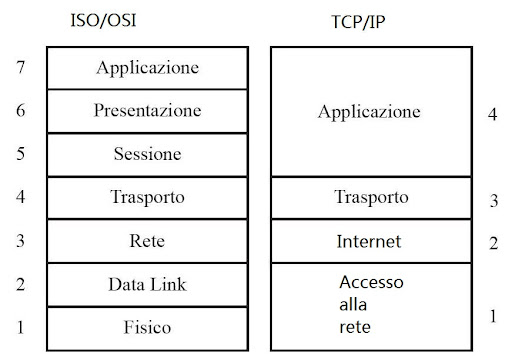
\includegraphics[scale=0.6]{stack-protocollari-a-confronto.jpg}
    \caption{\emph{ISO/OSI} VS \emph{TCP/IP}}
\end{figure}

\paragraph{Livelli dello stack protocollare ISO/OSI}
Esaminiamo il significato dei vari livelli dello stack \emph{ISO/OSI}:
\begin{enumerate}
    \item \emph{Fisico}: gestisce il trasferimento dei singoli bit
    \item \emph{Data link}: organizza l'instradamento dei frame attraverso una serie
    di commutatori;
    \item \emph{Rete}: instrada i pacchetti verso la rete del destinatario;
    \item \emph{Trasporto}: gestisce l'instradamento dei segmenti verso una
    specifica applicazione attiva nella rete di destinazione;
    \item \emph{Sessione}: gestisce sessioni di comunicazioni e la sincronizzazione
    dei flussi di dati (e.g. streaming audio-video);
    \item \emph{Presentazione}: consente alle applicazioni di interpretare il
    significato dei dati gestendo parametri come compressione e cifratura;
    \item \emph{Applicazione}: fornisce alle applicazioni i mezzi per scambiarsi
    messaggi;
\end{enumerate}
Il motivo per cui nello \emph{stack TCP/IP} mancano i livelli \emph{sessione} e
\emph{presentazione} è che possono essere inclusi nei protocolli di
\emph{livello Applicazione};

\paragraph{Incapsulamento}
La stratificazione dei protocolli consente di rendere modulare la comunicazione in
rete. La modularità porta numerosi vantaggi, tra i quali:
\begin{itemize}
    \item \emph{Trasparenza}: una modifica ai protocolli di un livello è trasparente
    ai protocolli di altri livelli;
    \item \emph{Semplificazione}: il modello a strati permette di identificare più
    facilmente i diversi componenti di un sistema che altrimenti risulterebbe
    estremamente complesso;
\end{itemize}

\paragraph{Comunicazione tra livelli}
Ogni \emph{livello} (\emph{layer}) fornisce un servizio al \emph{livello}
superiore, il quale vede il \emph{livello} inferiore come una black-box della
quale sfruttarne i servizi.

\begin{figure}[h]
    \centering
    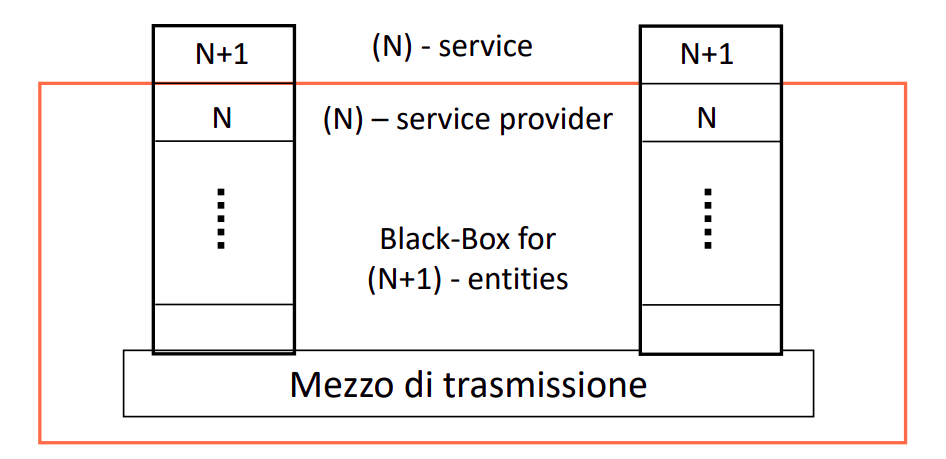
\includegraphics[width=\textwidth]{modularizzazione-protocolli.png}
    \caption{Modularizzazione dei servizi}
\end{figure}\noindent
La comunicazione tra livelli avviene mediante \emph{\gls{glos:SAP}}, in
modo che un servizio del \emph{livello N} è offerto all'entità di
\emph{livello N+1} attraverso un'interfaccia di programmazione detta
appunto \emph{SAP}. Lo scambio di informazioni tra entità dello stesso
\emph{livello}, invece, è regolata dai \emph{protocolli}.

\begin{figure}[h]
    \centering
    \subfloat[\emph{Comunicazione tra servizi di diverso livello}]{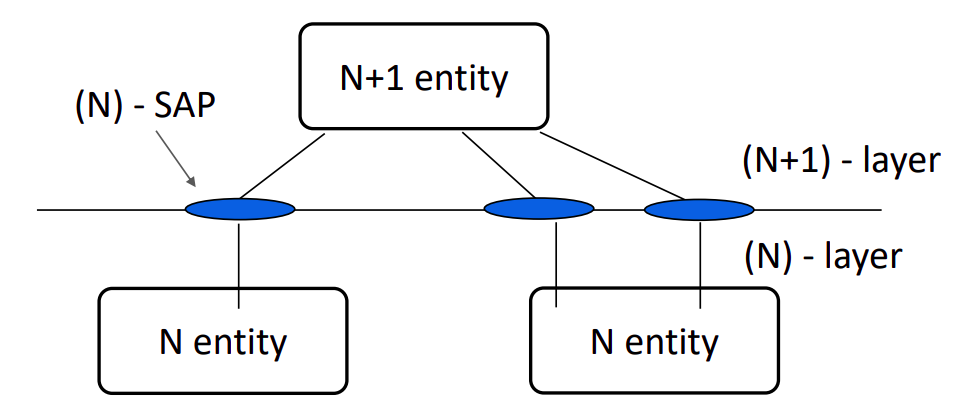
\includegraphics[scale=0.25]{comunicazione-servizi-diverso-livello.png}}
    \hfill
    \subfloat[\emph{Comunicazione tra servizi dello stesso livello}]{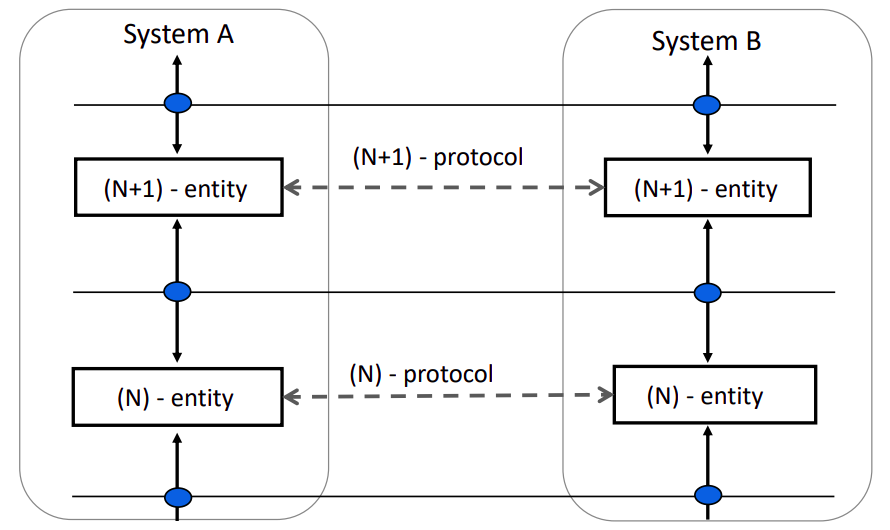
\includegraphics[scale=0.25]{comunicazione-servizi-stesso-livello.png}}
    \caption{Comunicazioni tra servizi}
\end{figure}

\paragraph{Data unit}
La suddivisione in livelli dei servizi cambia il modo in cui i dati, o meglio le
\emph{\gls{glos:DU}} da trasmettere vengono trattate. In un sistema a livelli, i dati da trasmettere da un \emph{livello
N} costituiscono un \emph{N-\gls{glos:SDU}} (\emph{SDU} di \emph{livello N}).

A questo \emph{N-SDU} il \emph{livello} aggancia il proprio \emph{N-\gls{glos:PCI}}
(\emph{PCI} di \emph{livello N}), cioè aggiunge le informazioni necessarie al
\emph{protocollo} per funzionare. Il risultato è un \emph{N-\gls{glos:PDU}}
(\emph{PDU} di \emph{livello N}).

Ogni \emph{livello} considera il \emph{PDU} del livello superiore come una busta
chiusa. Cioè, l'\emph{N-PDU} è l'\emph{SDU} di \emph{livello N-1} e aggiungendo
l'\emph{(N-1)-PCI} all'\emph{(N-1)-SDU} si ottiene l'\emph{(N-1)-PDU}.

\paragraph{Trasmissione e ricezione}
Nel momento della trasmissione i dati veri e propri vengono progressivamente
imbustati insieme al \emph{PCI} di livello, partendo dal \emph{livello Applicativo}
e scendendo fino al \emph{Fisico}. Per la ricezione, invece, si segue il processo
inverso, quindi partendo dal \emph{Fisico} e salendo all'\emph{Applicativo} ogni
\emph{livello} rimuove il proprio \emph{PCI}.

\begin{figure}[h]
    \centering
    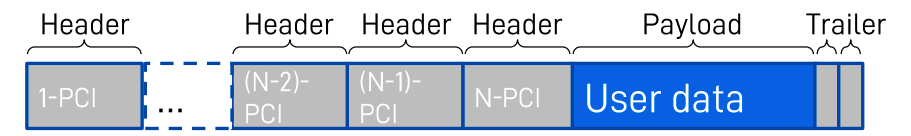
\includegraphics[width=\textwidth]{schema-di-un-PDU.png}
    \caption{Rappresentazione di un \emph{PDU} alla fine del processo di imbustamento}
\end{figure}\noindent
Le \emph{DU} possono essere:
\begin{itemize}
    \item \emph{Segmentate}: se la dimensione dei dati eccede il limite massimo,
    possono essere suddivisi in più \emph{SDU};
    \item \emph{Assemblate}: per evitare inefficienze, più \emph{N-SDU} di piccola
    dimensione possono essere aggregate in un unico \emph{N-SDU} e trasmesse insieme;
    \item \emph{Ri-assemblate}: è il processo inverso della \emph{segmentazione};
\end{itemize}

\paragraph{Le PDU di livello}
A seconda del \emph{livello} in cui si trovano le \emph{PDU} possono avere nomi
diversi:
\begin{itemize}
    \item \emph{Applicazione}: messaggi;
    \item \emph{Trasporto}: segmenti;
    \item \emph{Rete}: pacchetti;
    \item \emph{Data link}: frame;
\end{itemize}